\documentclass[9pt]{beamer}
\usepackage[utf8]{inputenc}
\usepackage[spanish]{babel}
\usepackage{mathtools}
\usepackage{amsmath}
\usepackage{amsfonts}
\usepackage{amssymb}
\usepackage{graphicx}
\usepackage{lipsum}
\usepackage{ragged2e}
\usepackage{hyperref}
\usepackage{float}
\usepackage{url}
\usepackage{tikz}
\usepackage{relsize}
\graphicspath{{./imgs/}}
\usetheme{JuanLesPins}
\setbeamertemplate{navigation symbols}{}
\newtheorem{teorema}{Teorema}
\newtheorem{corolario}{Corolario}
\newcommand{\celda}[1]{
	\begin{minipage}{2.5cm}
		\vspace{5mm}
		#1
		\vspace{5mm}
	\end{minipage}
}
\newcommand{\norm}[1]{\left\Vert#1\right\Vert}
\newcommand{\abs}[1]{\left\vert#1\right\vert}
\newcommand{\pre}[1]{\left\langle#1\right\rangle}
\newcommand{\set}[1]{\left\{#1\right\}}
\newcommand{\RR}{\mathbb{R}}
\newcommand{\NN}{\mathbb{N}}
\newcommand{\ZZ}{\mathbb{Z}}
\newcommand{\vecSpace}{ $V$ }
\newcommand{\ttt}{\textbf{\emph{t}}}
\newcommand{\sss}{\textbf{\emph{s}}}
\newcommand{\xx}{\textbf{\emph{x}}}
\newcommand{\yy}{\textbf{\emph{y}}}
\newcommand{\vv}{\textbf{\emph{v}}}
\newcommand{\ww}{\textbf{\emph{w}}}
\newcommand{\zz}{\textbf{\emph{z}}}
\newcommand{\ccc}{\textbf{\emph{c}}}
\newcommand{\topSpace}{X}
\newcommand{\topSpaceY}{Y}
\newcommand{\aaa}{\textbf{\emph{a}}}
\newcommand{\bbb}{\textbf{\emph{b}}}
\newcommand{\uu}{\textbf{\emph{u}}}
\newcommand{\barx}{\bar{x} }
\newcommand{\barxx}{\bar{\mathbf{x}}}
\newcommand{\lambdaa}{\boldsymbol{\mathbf{\lambda}}}
\newcommand{\dd}{\textbf{\emph{d}}}
\newcommand{\pp}{\textbf{\emph{p}}}
\newcommand{\bb}{\textbf{\emph{b}}}

\author[]{Pedro Manuel Flores Crespo}
\title[Trabajo Fin de Grado]{Teoremas de la alternativa, optimización convexa, valoración de activos financiero y procesamiento de nubes de puntos generadas por escáner láser.}
\date{8-9 julio de 2020} 

\AtBeginSection[]
{
	\begin{frame}<beamer>{Contenido}
		\tableofcontents[currentsection,currentsubsection]
	\end{frame}
}


\begin{document}
	
	\begin{frame}
		\maketitle
	\end{frame}

	\begin{frame}{Índice}
		\tableofcontents
	\end{frame}

	\section[Teoremas de la alternativa, optimazión convexa y valoración de activos financieros]{Teoremas de la alternativa, optimazión convexa y valoración de activos financieros.}

	\begin{frame}{Desarrollo}
	\begin{figure}[h!]
		%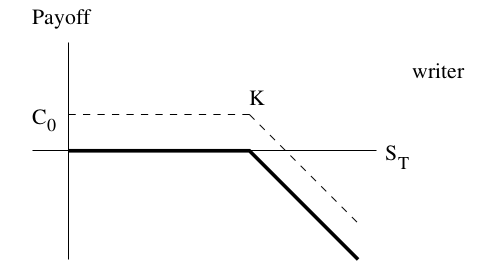
\includegraphics[width=1\linewidth]{Writer_call}
		\centering
		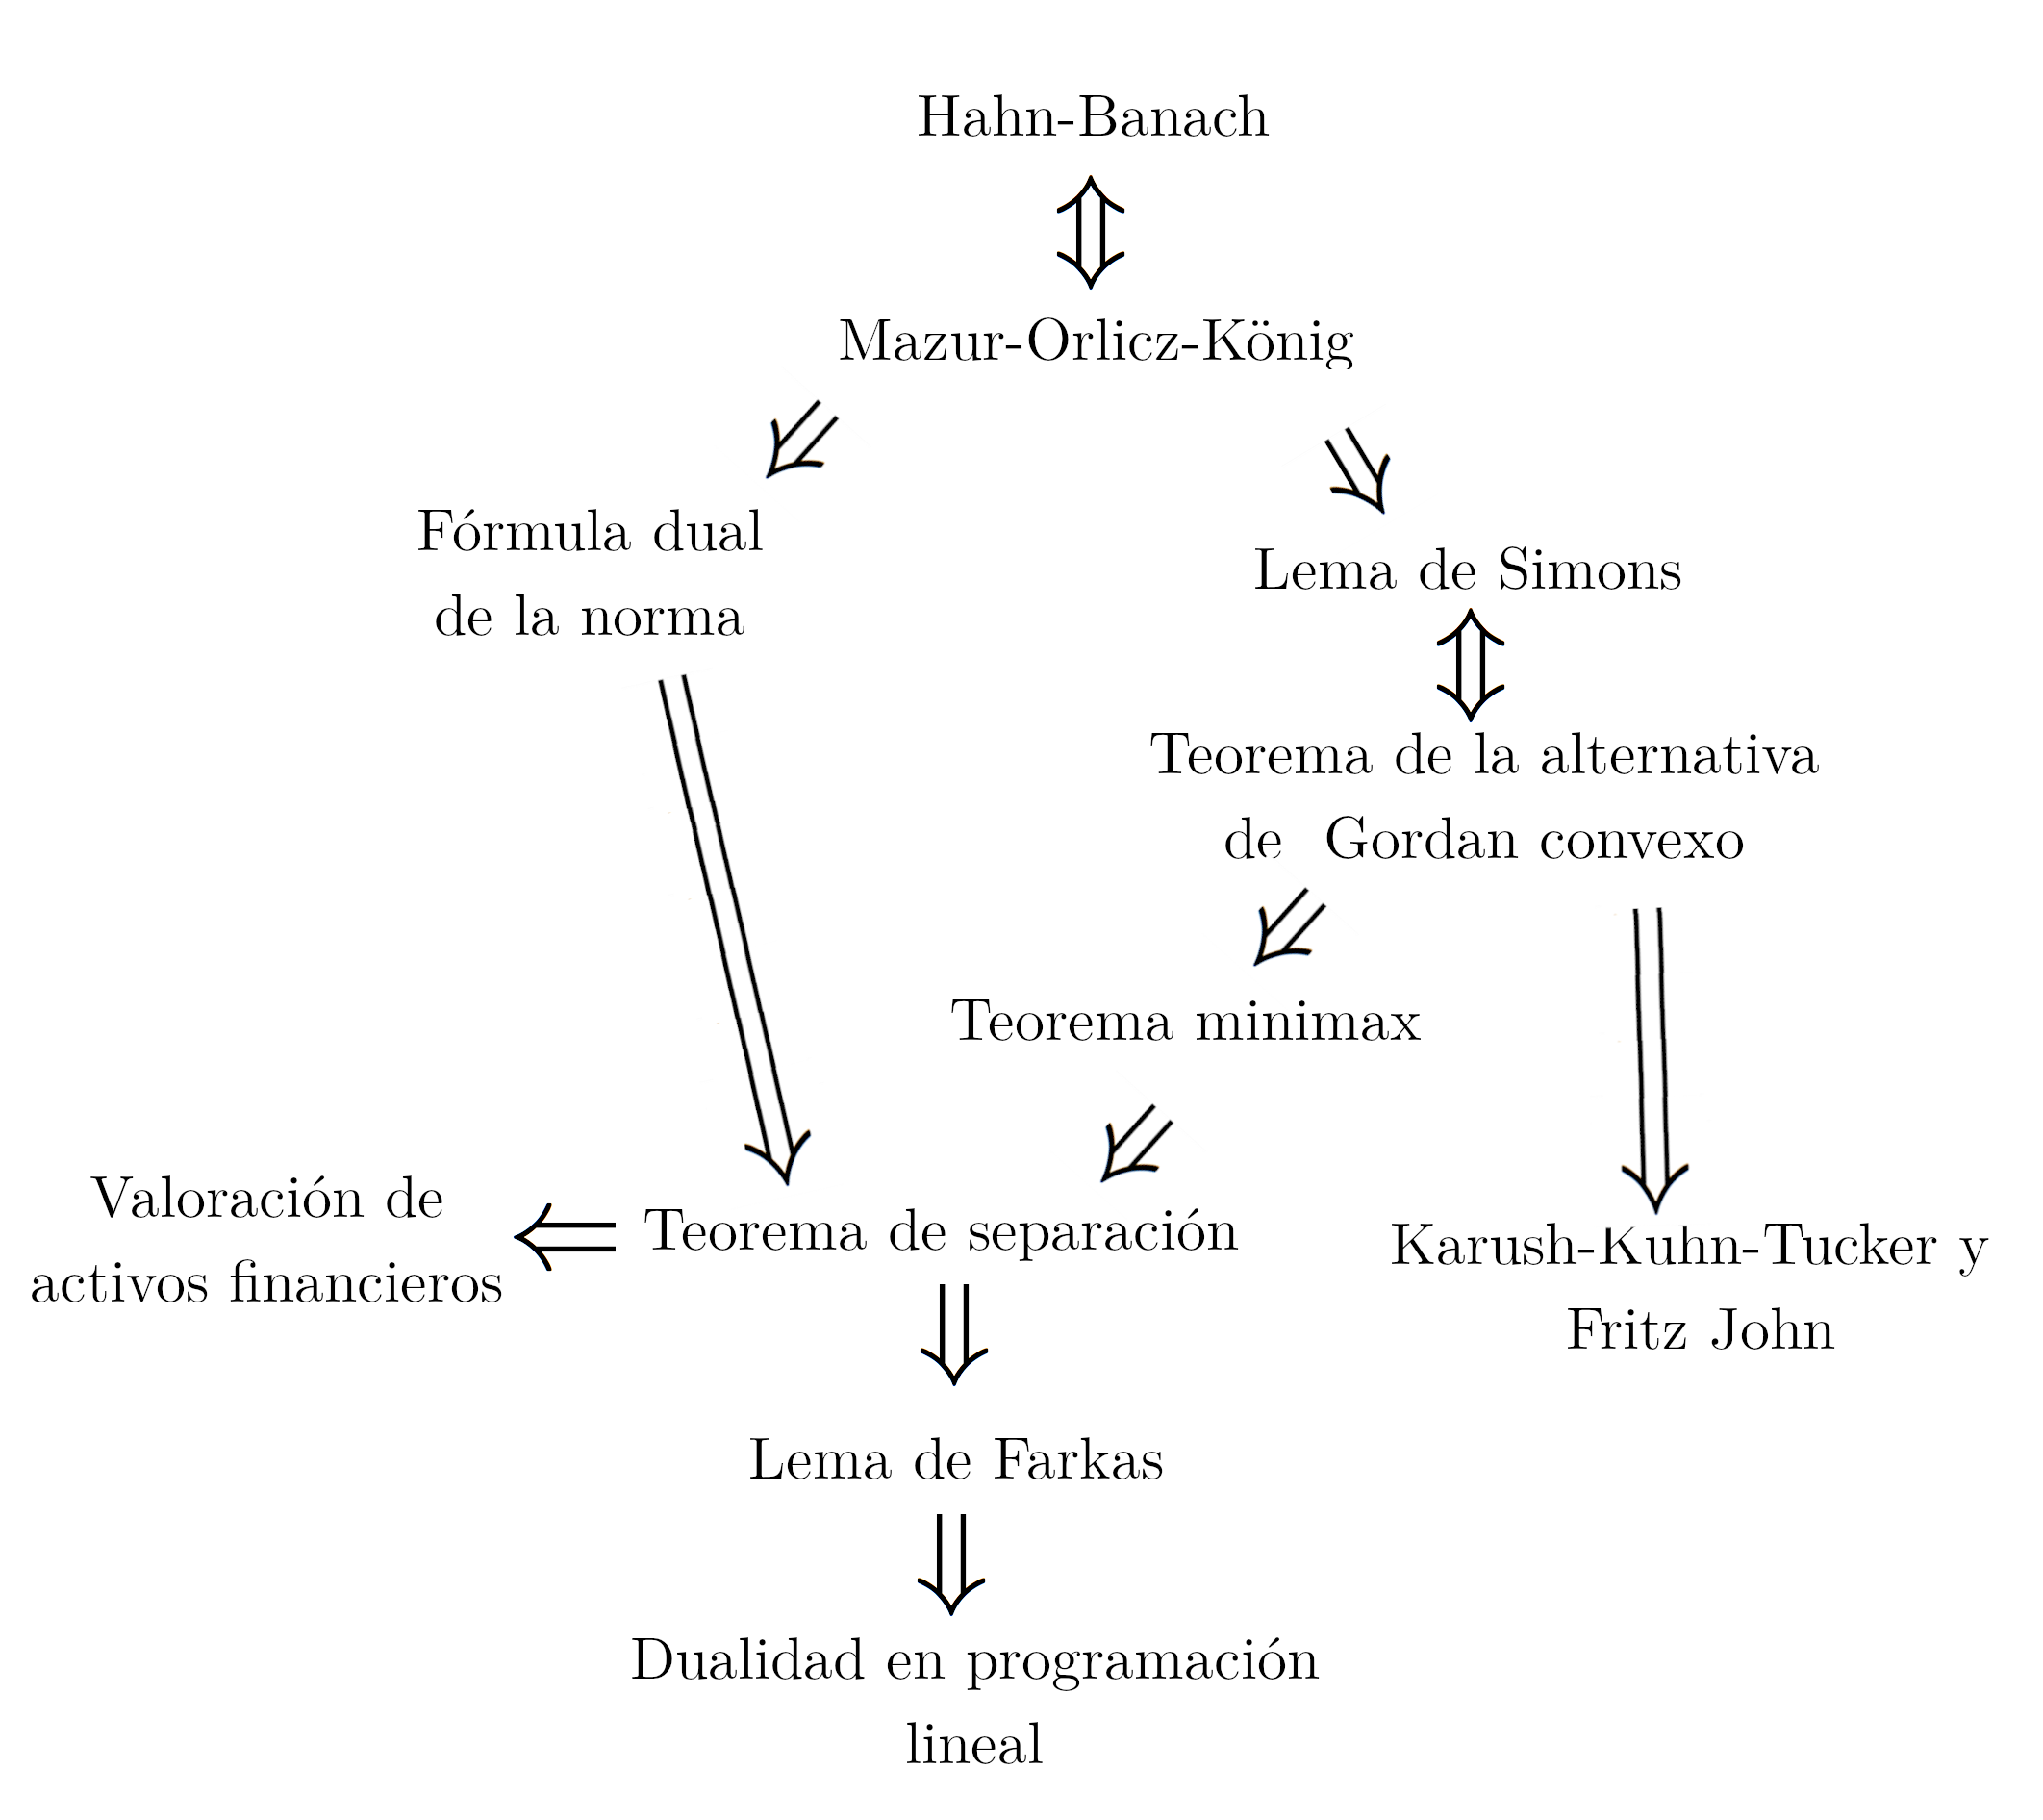
\includegraphics[width=0.8\linewidth]{esquema}
		%\caption{Teorema de Hahn-Banach.}
	\end{figure}
	\end{frame}


	\subsection{Hahn-Banach y Mazur-Orlicz-König}
		\begin{frame}[fragile]{}
			\begin{columns}
				\column{0.5\textwidth}
				\begin{teorema}[Hahn-Banach]
					Sea V un espacio vectorial y $P:V \rightarrow \RR$ un funcional sublineal. Entonces existe un funcional lineal $ L:\vecSpace \longrightarrow \RR $ tal que $ L \leq P $.
				\end{teorema}
			\begin{figure}[h!]
				%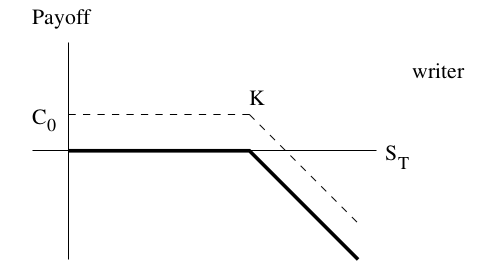
\includegraphics[width=1\linewidth]{Writer_call}
				\centering
				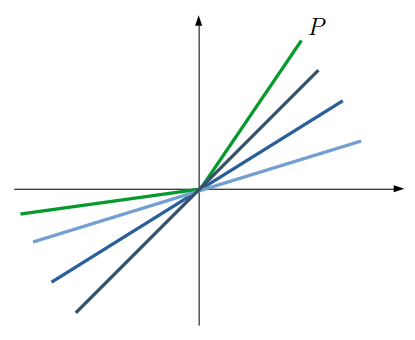
\includegraphics[width=0.8\linewidth]{H-B_2}
				\caption{Teorema de Hahn-Banach.}
			\end{figure}
				\column{0.5\textwidth}
				\begin{teorema}[Mazur-Orlicz-König]
						Sea\vecSpace un espacio vectorial y $P:\vecSpace \rightarrow \RR$ un funcional sublineal.  Sea $ D $ un subconjunto no vacío y convexo de $ V $. Entonces existe un funcional $ L: \vecSpace \longrightarrow \RR $ lineal tal que $ L \leq P $ e $ \inf_D L = \inf_D P $.
				\end{teorema}
			\begin{figure}[h!]
				%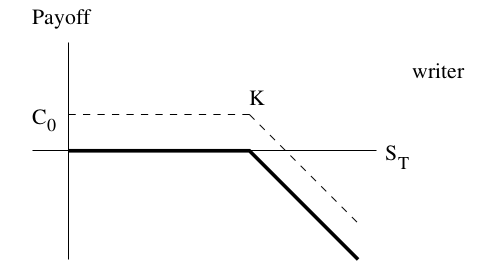
\includegraphics[width=1\linewidth]{Writer_call}
				\centering
				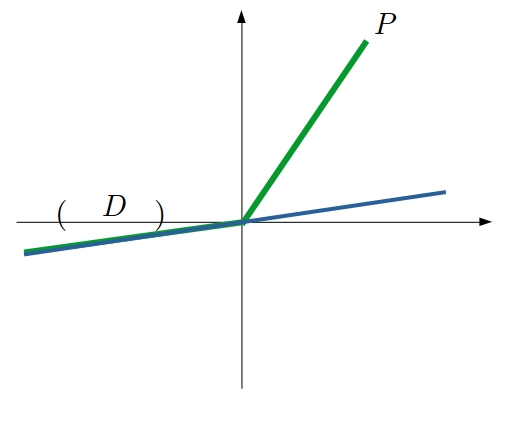
\includegraphics[width=0.8\linewidth]{M-O-K}
				\caption{Teorema de Mazur-Orlicz-König.}
			\end{figure} 
			\end{columns}
		\end{frame}

	\subsection{Toerema de la alternativa de Gordan}
		\begin{frame}[fragile]
			\begin{teorema}[Teorema de la alternativa de Gordan]\label{GordanClasic}
				Dados $N, M \in \NN   $, sean $ \{\xx_1,...\xx_N\}$ con $ \xx_i \in \RR^M \text{ para } i=1,...,N$. Entonces una, y solo una, de la siguientes afirmaciones se cumple:
				
				\begin{itemize}
					\item[i*)] $ \exists \mathbf{t} \in \Delta_N $ tal que  $  0 = \displaystyle \sum_{i=1}^{N}{t_i \xx_i}$.
					\item[ii*)] $ \exists \yy \in \RR^M $ tal que cumple $ \displaystyle \max_{i=1,...,N} \langle \yy, \xx_i \rangle < 0 $.
				\end{itemize}
			\end{teorema}
			\begin{columns}
				\column{0.5\textwidth}
				\begin{figure}[h!]
					%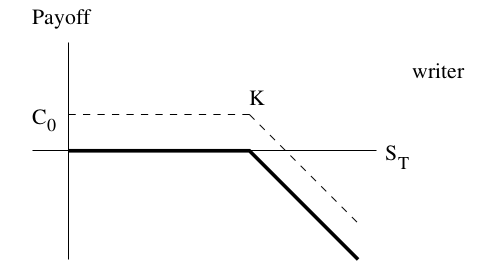
\includegraphics[width=1\linewidth]{Writer_call}
					\centering
					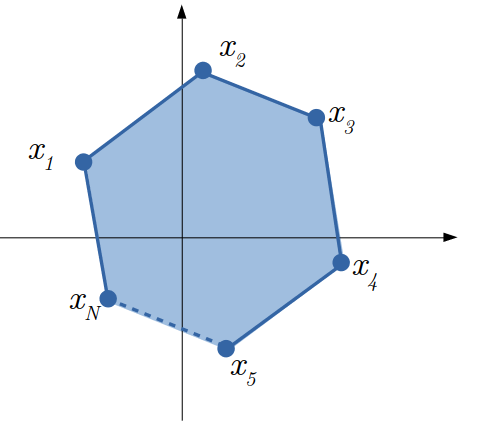
\includegraphics[width=0.7\linewidth]{Gordan-i*}
					\caption{Alternativa i*).}
				\end{figure}
				\column{0.5\textwidth}
				\begin{figure}[h!]
					%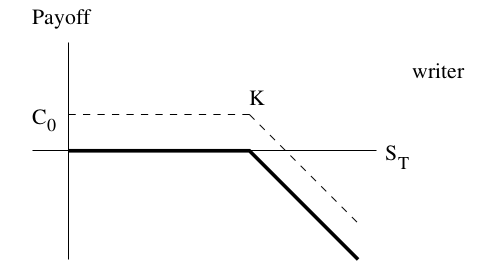
\includegraphics[width=1\linewidth]{Writer_call}
					\centering
					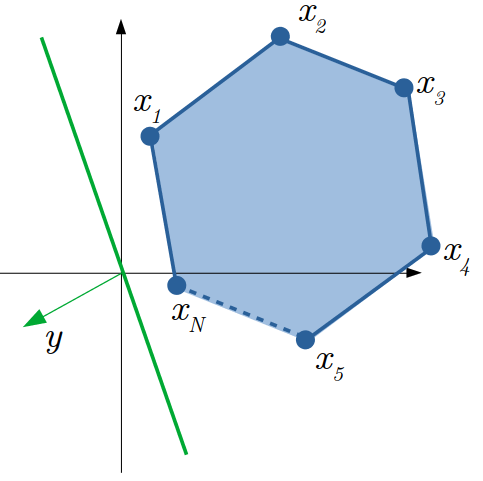
\includegraphics[width=0.7\linewidth]{Gordan-ii*}
					\caption{Alternativa ii*).}
				\end{figure} 
			\end{columns}
	
		\end{frame}
	\subsection{Optimización}
	\begin{frame}{}
		Nuestro objetivo ahora es encontrar soluciones a problemas del siguiente tipo:
		
		\begin{equation}\label{probMin}
		\begin{cases}
		\displaystyle\inf_{\xx\in D} f(\xx)\\
		\begin{split}
		\text{s.a } g_1(\xx) &\leq 0 \\
		&\vdots \\
		g_N(\xx) &\leq 0
		\end{split}
		
		\end{cases} 
		\end{equation}
		\begin{teorema}[Teorema de Fritz John]\label{FritzJohn}
			Supongamos que el problema (\ref{probMin}) tiene un mínimo local en $ \barxx \in D $. Si las funciones $ f, g_i $ con $ i \in I(\barxx) $ son diferenciables en $ \barxx $ entonces existen $ \lambda_0, \lambda_i \in \RR^+ $ para $ i \in I(\barxx) $, no todas cero, que satisfacen:
			\[
			\lambda_0 \nabla f(\barxx) + \sum_{i \in I(\barxx)} \lambda_i \nabla g_i(\barxx) = 0.
			\]
		\end{teorema}
		
		\begin{itemize}
			\item Fritz-John + Condicón de Mangasarian-Fromovitz = Karush-Kuhn-Tucker.
		\end{itemize}
	\end{frame}

	\subsection{Minimax}
	\begin{frame}[fragile]
		A rasgos generales y a modo introductorio, podemos decir que un teroema minimax es un resultado que afirma, bajo ciertas hipótesis, que:
		\[
		\inf_{y \in Y} \sup_{x \in X} f(x,y) \leq \sup_{x \in X} \inf_{y \in Y} f(x,y),
		\] 
		\begin{teorema}\label{MinMax}
			Sean $ \topSpace,\hspace{0.5mm} \topSpaceY $ subconjuntos convexos de sendos espacios vectoriales (no tienen que ser el mismo) tal que $ \topSpace $ está dotado de una topología que lo hace compacto. Supongamos además que $ f:  \topSpace \times \topSpaceY \longrightarrow \RR $ es:
			\begin{itemize}	
				\item[i)] cóncava y superiormente semicontinua en $ \topSpace $ y
				\item[ii)] convexa en $ \topSpaceY $.
			\end{itemize}
			Entonces:
			\begin{equation*}\label{eqMinMax}
			\inf_{y \in Y} \max_{x \in X} f(x,y) = \max_{x \in X} \inf_{y \in Y} f(x,y).
			\end{equation*}
		\end{teorema}
	\end{frame}

	\subsection{Separación de convexos}
	\begin{frame}
		\begin{teorema}\label{separacion1}
			Sean $ N\in \NN $ y $ A,B $ subconjuntos convexos de $ \RR^N $ tal que $ A $ es cerrado, $ B $ es compacto y $ A \cap B = \emptyset$. Entonces existe $ \xx_0 \in \RR^N $ tal que
			\[
			\sup_{\aaa \in A} \langle \xx_0,\aaa\rangle < \inf_{\bbb\in B} \langle \xx_0,\bbb\rangle.
			\]
		\end{teorema}
		\begin{figure}[h!]
			\begin{center}
				\begin{tikzpicture}[thick,fill opacity=0.5]
				\filldraw[fill=red][rotate = 30] (0:4cm) ellipse (8mm and 5 mm);
				\filldraw[fill=green] (1cm:1cm) circle (12mm);
				\draw (-1,3) -- (5,0);
				%\node at (0.9cm,0.6cm) {\large A};
				%\node at (3.5cm,2.1cm) {\large B};
				\end{tikzpicture}
			\end{center}
			\caption{Situación de teoremas de separación}
			\label{prueba}
		\end{figure}
	%	\begin{corolario}\label{coroSep}
	%		Sean $ N \in \NN $, $ L \leq \RR^N $ subespacio vectorial y $ K \subset \RR^N $ un subconjunto compacto y convexo tales que $ L \cap K = \emptyset $. Entonces, $ \exists \xx_0 \in \RR^N $ tal que si $ \yy \in L $, entonces $ \langle \xx_0, \yy\rangle = 0 $ y 
	%		\[
	%		0 < \inf_{ \xx \in K} \langle \xx_0, \xx\rangle.
	%		\]
	%	\end{corolario} 
	
	\end{frame}

	\subsection{Valoración de activos financieros}
	\begin{frame}{Preliminares financieros}
		\begin{itemize}
			 \item Definición de activo y opción de compra (europea). Opciones \textit{call} y \textit{put}.
			 \[
			 C_T = \max\{S_T-K, 0\} = \left[S_T - K\right]^+
			 \] 
			 \item Principio de arbitraje.
		\end{itemize}
		\begin{columns}
			\column{0.5\textwidth}
			\begin{figure}[h!]
				%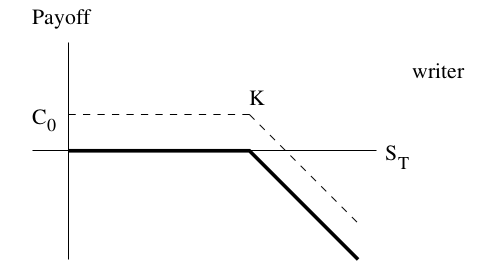
\includegraphics[width=1\linewidth]{Writer_call}
				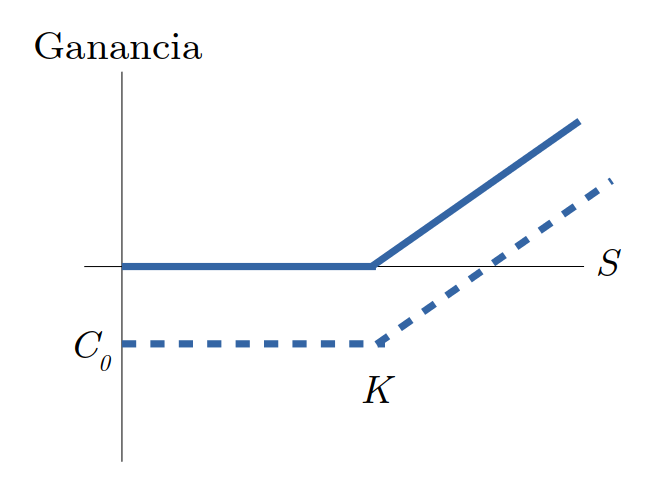
\includegraphics[width=0.8\linewidth]{Buyer_call_mio}
				\caption{Ganancia propietario opción \textit{call}.}
			\end{figure}
			\column{0.5\textwidth}
			\begin{figure}[h!]
				%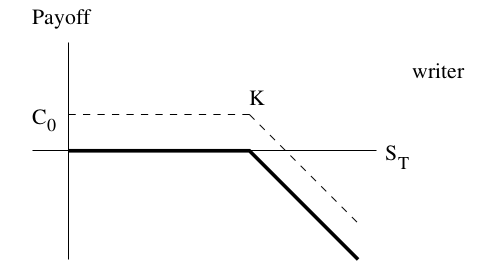
\includegraphics[width=1\linewidth]{Writer_call}
				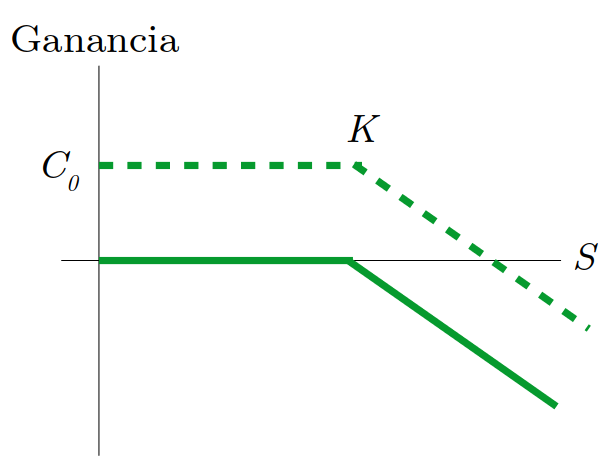
\includegraphics[width=0.8\linewidth]{Writer_call_mio}
				\caption{Ganancia vendedor opción \textit{call}}
			\end{figure} 
		\end{columns}
	
	\end{frame}

	\begin{frame}{Martingalas}
		Un proceso $ \mathbb{F} $-adaptado $ M = (M_t)_{t\in \mathbb{T}} $ es una $ ( \mathbb{F},P)$-mar\-tingala si $ E(|M_t|) < \infty $ para todo $ t \in \mathbb{T} $ y 
		\[
		E(M_{t+1}|\mathcal{F}_t) = M_t \textit{ para todo } t \in \mathbb{T}\setminus\{T\}.
		\]
		\begin{teorema}(Primer reorema fundamental de asignación de precios)\label{VIABLEiofEMM}
			Un modelo de mercado discreto es viable si, y solo si, existe una medida de martingala equivalente para $ S $.
		\end{teorema}
	\end{frame}

	\begin{frame}{Precio de una opción de compra \textit{call}. Modelo binomial}
		
	El precio el instante $ t \in \mathbb{T} $ viene dado por
	\[
	S_t =  \begin{cases}
	S_{t-1}(1+u) & \text{ con probabilidad } p\\
	S_{t-1}(1+d) & \text{ con probabilidad } 1-p
	\end{cases} \text{ donde }-1 < d <u.
	\]
		
	La medida martingala equivalente $ Q $ es:
	\[
	\begin{cases}
	Q (\frac{S_t}{S_{t-1}} = 1+u ) =  q \\
	Q (\frac{S_t}{S_{t-1}} = 1+d ) =  1-q
	\end{cases}
	\]
	con $ q = \frac{r-d}{u-d} $ con $ d < r < u $. El valor de una opción viene dado por
	\begin{equation*}
	V_0(C_T) = (1+r)^{-T} \sum_{v=A}^{T}\binom{T}{v}q^v(1-q)^{T-v}\left[S_0(1+u)^v(1+d)^{T-v}-K\right],
	\end{equation*}
	donde $ A $ denota el primer entero $ k $ que cumple $ S_0(1+u)^k(1+d)^{T-k} > K $
	
	\end{frame}
	
	\begin{frame}{Estudio del valor en función de algunos de sus parámetros}
		\begin{columns}
			\column{0.5\textwidth}
			\begin{figure}[h!]
				%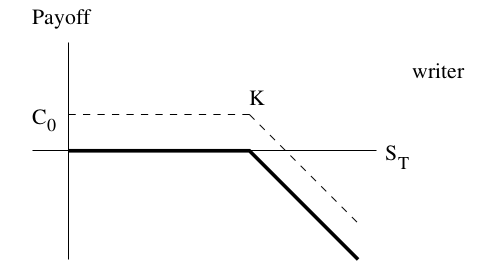
\includegraphics[width=1\linewidth]{Writer_call}
				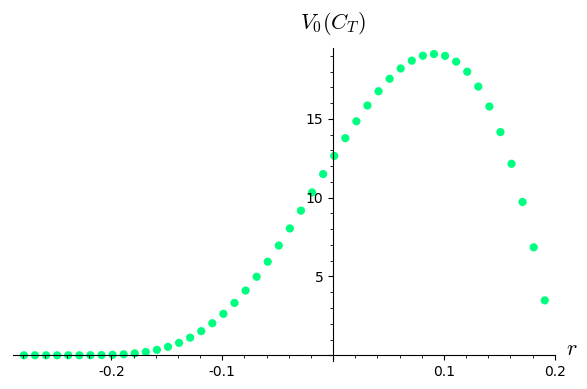
\includegraphics[width=1\linewidth]{value_r}
				\caption{Variación en función del valor de $ r $ ($ d= -0.28 $, $ u=0.2 $).}
			\end{figure}
			\column{0.5\textwidth}
			\begin{figure}[h!]
				%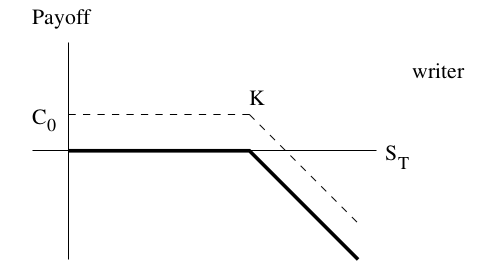
\includegraphics[width=1\linewidth]{Writer_call}
				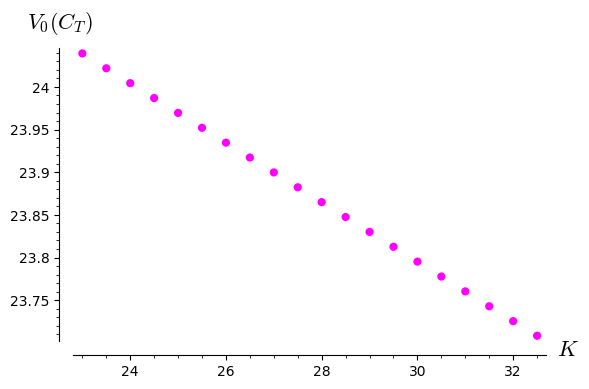
\includegraphics[width=1\linewidth]{value_K}
				\caption{Variación en función del valor de $ K $.}
			\end{figure} 
		\end{columns}
	\end{frame}
	
	\section[Procesamiento de nubes de puntos generadas por escáner láser]{Procesamiento de nubes de puntos generadas por escáner láser.}

	\subsection{Problema a resolver}
	\begin{frame}
		\begin{itemize}
			\item Interés del digitalizado 3D.
			\item Cauce habitual de trabajo:
			\begin{itemize}
				\item Alinear: expresar todas las tomas respecto al mismo sistema de referencia.
				\item Fusionar: eliminar puntos ``repetidos''.
				\item Triangular: construir malla de triángulos.
			\end{itemize}
		\end{itemize}
	\begin{columns}
		\column{0.5\textwidth}
		\begin{figure}[h!]
			%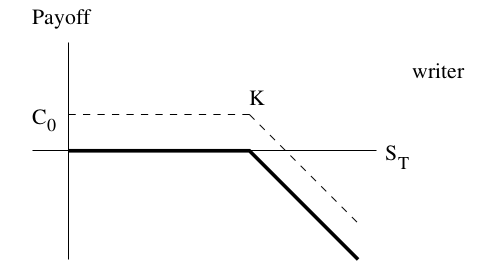
\includegraphics[width=1\linewidth]{Writer_call}
			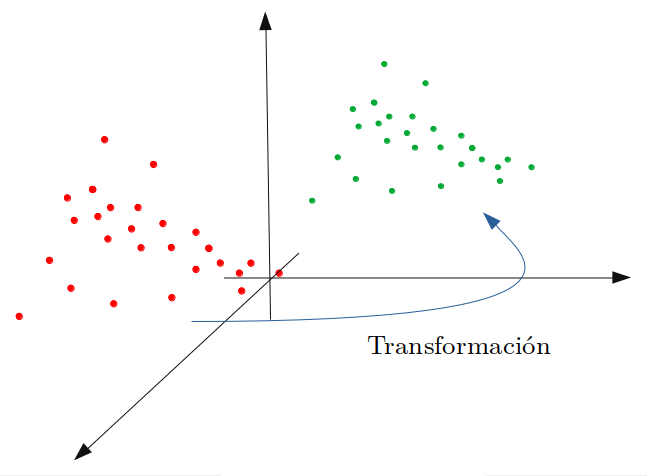
\includegraphics[width=1\linewidth]{Ej_Alineado_1}
			\caption{Nubes de puntos sin alinear.}
		\end{figure}
		\column{0.5\textwidth}
		\begin{figure}[h!]
			%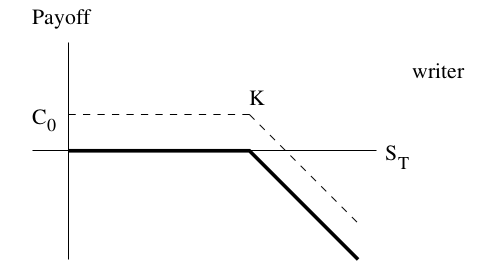
\includegraphics[width=1\linewidth]{Writer_call}
			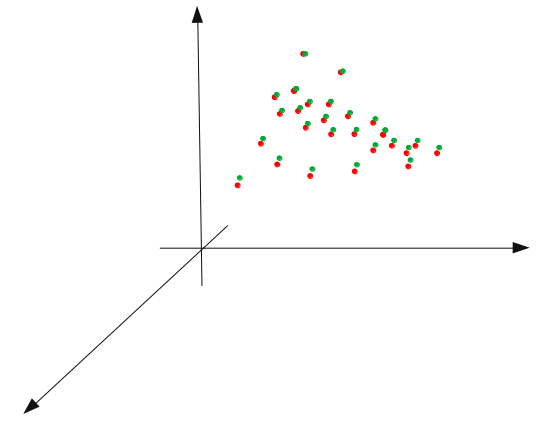
\includegraphics[width=1\linewidth]{Ej_Alineado_2}
			\caption{Nubes de puntos alineadas.}
		\end{figure} 
	\end{columns}

	\end{frame}
	\subsection{ICP}
	\begin{frame}
		\begin{itemize}
			\item Uso de cuaternios para expresar las rotaciones. 
			\item Para minimizar la distancia (euclidea) entre el conjunto de puntos $ P $ a alinear con el modelo $ X $, calculamos los vectores propios de 
		\end{itemize}
	
		\begin{equation}\label{matCov}
		M  =
		\begin{pmatrix}
		tr(\Sigma_{px}) & \Delta^t \\
		\Delta & \Sigma_{px} + \Sigma_{px}^t + tr(\Sigma_{px})I_3\\
		\end{pmatrix}, 
		\end{equation}
		donde 
		\[
		\Sigma_{px} = \frac{1}{N_p}\sum_{i=1}^{N_p} \lbrack (p_i-\bar{\pp})(x_i - \bar{\xx})^t\rbrack, \]
		\[A_{ij} = (\Sigma_{px}-\Sigma_{px}^t)_{ij} \quad i,j \in \lbrace 0,1,2 \rbrace,\]
		y 
		\[\Delta = \begin{pmatrix}
		A_{12} & A_{20} & A_{01}  \\
		\end{pmatrix}. \]
		
		El cuaternio que representa la rotación viene dado por el vector propio asociado al mayor valor propio de $ M $ y la traslación por el vector $ \bb = R\bar{\pp}  + \bar{\xx} $. \\
		
		El algoritmo ICP intenta minimizar la distancia entre los puntos más cercanos.
	
	\end{frame}

	\begin{frame}{Problemas del método ICP}
		\begin{itemize}
			\item Convergencia local $ \Longrightarrow $ Prealinear.
			\begin{columns}
				\column{0.3\textwidth}
				\begin{figure}[h!]
					%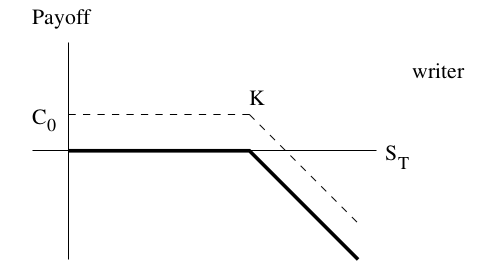
\includegraphics[width=1\linewidth]{Writer_call}
					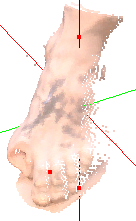
\includegraphics[width=0.6\textwidth]{prueba_ICP_2_3_1} 
					\caption{Conjunto (1) con $ 7\,042 $ puntos.}
				\end{figure}
				\column{0.3\textwidth}
				\begin{figure}[h!]
					%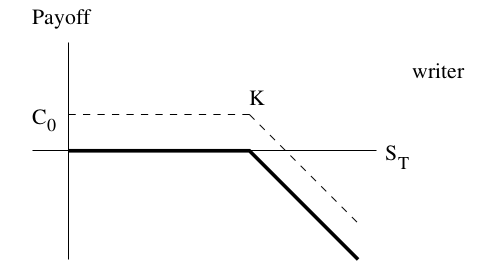
\includegraphics[width=1\linewidth]{Writer_call}
					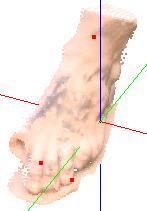
\includegraphics[width=0.6\textwidth]{prueba_ICP_2_3_2}
					\caption{Conjunto (2) con $ 8\,334 $ puntos.}
				\end{figure} 
				\column{0.0001\textwidth}
				\[
				\mathlarger{\Longrightarrow}
				\]
				\column{0.3\textwidth}
				\begin{figure}[h!]
					%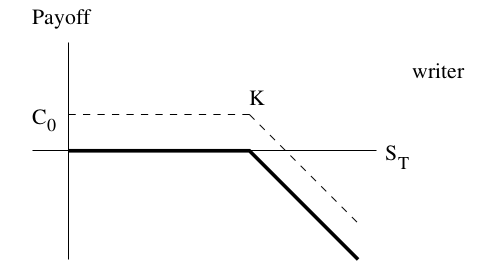
\includegraphics[width=1\linewidth]{Writer_call}
					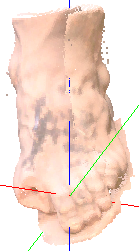
\includegraphics[width=0.6\textwidth]{prueba_ICP_2_3_3}
					\caption{Tomas prealineadas.}
				\end{figure} 
			\end{columns}
		
		\end{itemize}
	
	\end{frame}

	\begin{frame}{Problemas del método ICP}
		\begin{columns}
			\column{0.5\textwidth}
			\begin{table}[h!]
				\centering
				\begin{tabular}{| c | c | c | c |} 
					\hline
					It. & D. antes (mm)  & D. después (mm) & Seg. \\
					\hline
					1 & 21.2000 & 18.1299 & 62.8672\\		 
					2 & 16.7174 &  15.8707 &  62.7888\\	
					3 & 15.1625 & 14.4617  & 62.8636\\
					4 & 13.9753 &  13.7418 & 63.059\\
					5 &  13.6518 &  13.6071 & 62.8259\\
					\hline
				\end{tabular}
				\caption{Resultados ajuste mediante ICP.}
			\end{table}
			\column{0.5\textwidth}
			\begin{figure}[h!]
				%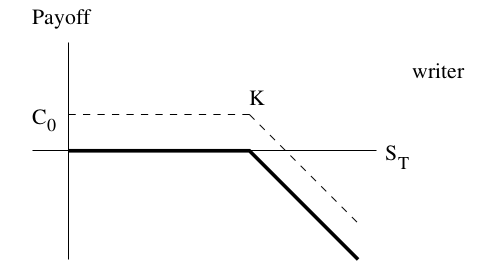
\includegraphics[width=1\linewidth]{Writer_call}
				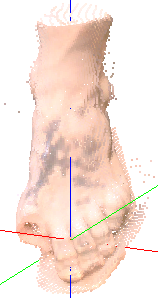
\includegraphics[width=0.4\textwidth]{prueba_ICP_2_3_5}
				\caption{Tomas alineadas.}
			\end{figure} 
		\end{columns}
		
		\begin{itemize}
			\item Orden cuadrático en tiempo $ \Longrightarrow $ Reducir el conjunto de puntos a los que aplicar el método.
		\end{itemize}
	\end{frame}
	\subsection{Mejoras ICP}
	\begin{frame}
		\justifying
		\begin{itemize}
			\item Para reducir el conjunto de puntos, detectamos puntos clave midiendo las variaciones de la normal (previo proceso de simplificado de la malla).
			
			\begin{figure}[h!]
				%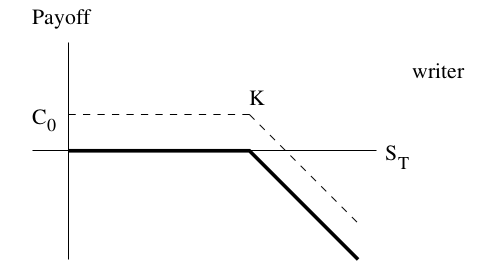
\includegraphics[width=1\linewidth]{Writer_call}
				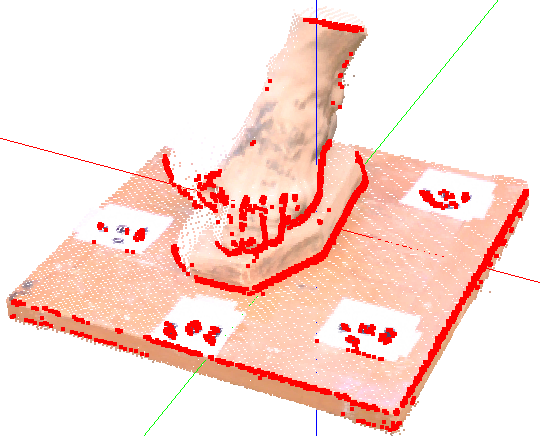
\includegraphics[width=0.4\textwidth]{desNormal-simp8}
				\caption{Puntos clave en la malla simplificada ($ 1\,885 $).}
			\end{figure} 
			
			\item Podemos tomar puntos clave en una toma o en las dos (con algunas consideraciones).
			\item En la segunda opción, se han reducido dos conjuntos de puntos de unos $ 80\,000 $ puntos a $ 1\,1142 $ y $ 2\,273 $ obteniendo resultados satisfactorios empleando 0.7 segundos por iteración.
		\end{itemize}
		
		
	\end{frame}

	\subsection{RANSAC}
	\begin{frame}
		\justifying
		EL algoritmo RANSAC (\textit{RAndom Sample Consensus}) es del tipo hipótesis-y-prueba y sirve para ajustar parámetros de un modelo matemático
		
		\begin{columns}
			\column{0.33\textwidth}
			\begin{figure}[h!]
				%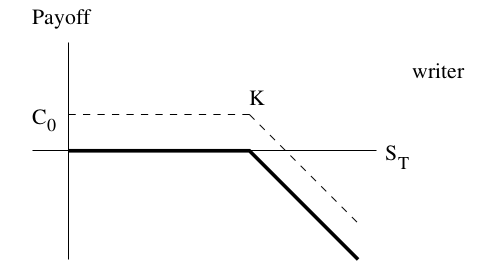
\includegraphics[width=1\linewidth]{Writer_call}
				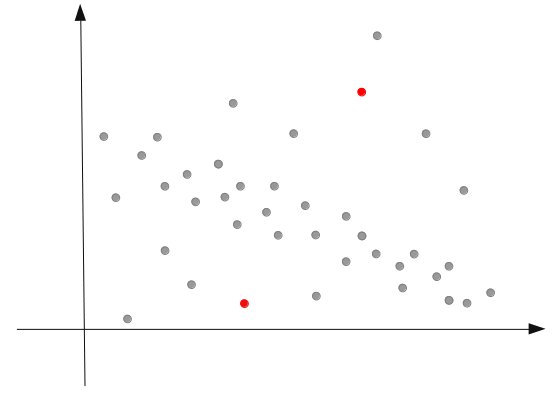
\includegraphics[width=1\linewidth]{ejRANSAC_10}
				\caption{Escogemos los puntos.}
			\end{figure}
			\column{0.33\textwidth}
			\begin{figure}[h!]
				%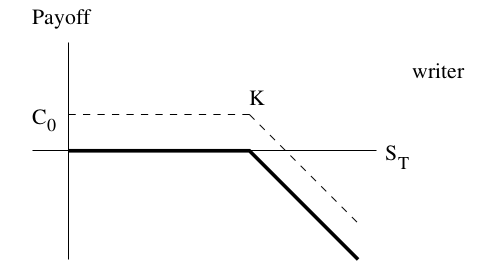
\includegraphics[width=1\linewidth]{Writer_call}
				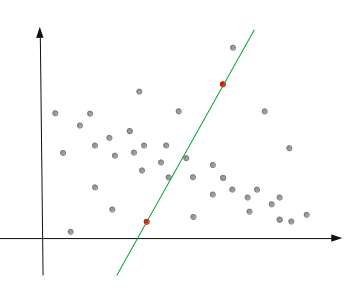
\includegraphics[width=1\linewidth]{ejRANSAC_11}
				\caption{Trazamos el modelo.}
			\end{figure} 
			\column{0.33\textwidth}
			\begin{figure}[h!]
				%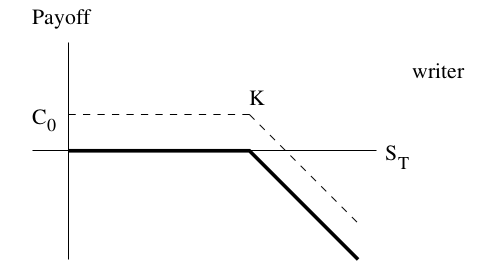
\includegraphics[width=1\linewidth]{Writer_call}
				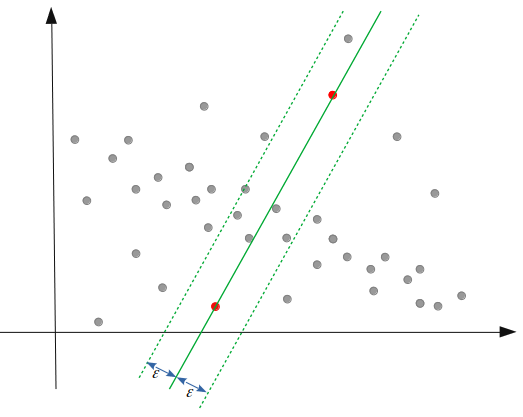
\includegraphics[width=1\linewidth]{ejRANSAC_12}
				\caption{Vemos cómo de bueno es.}
			\end{figure} 
		\end{columns}
		El número de iteraciones necesarias depende de los puntos necesarios para definir el modelo, la probabilidad para asegurar que encontramos uno adecuado y de la probabilidad de no estar en el modelo.
	\end{frame}	

	\begin{frame}{Aplicación en alineado}
	Usamos el algoritmo RANSAC para obtener los puntos de intersección entre planos y alineamos el modelo en base a esos puntos.
	\begin{figure}[h!]
		%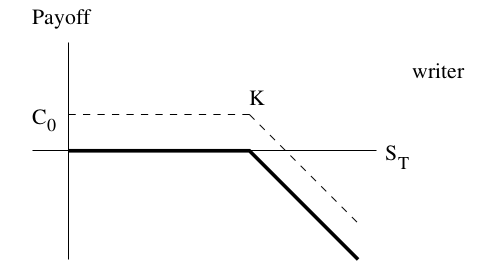
\includegraphics[width=1\linewidth]{Writer_call}
		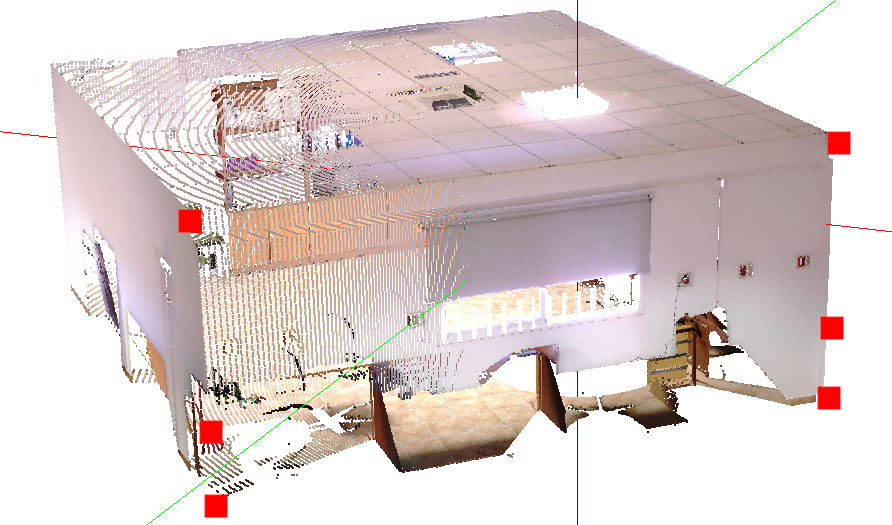
\includegraphics[width=0.7\linewidth]{inter0-pared+mesas}		
	\end{figure} 

	Problema $ \Longleftrightarrow $ se necesitan muchos planos para obtener resultados satisfactorios y que se puedan diferenciar fácilmente unos puntos de otros.
	
	\end{frame}

	\subsection{Banco de pruebas}
	\begin{frame}{Desarrollo del banco de pruebas}
		La aplicación para ver los resultados se ha hecho mediante \textit{Qt}, \textit{OpenGL} y \textit{C++}.
		\begin{figure}[h!]
			%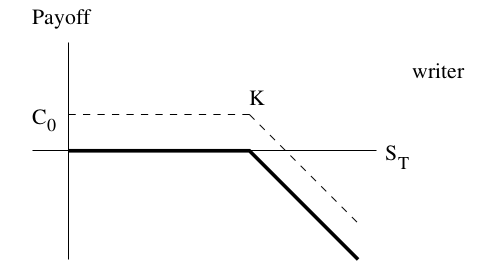
\includegraphics[width=1\linewidth]{Writer_call}
			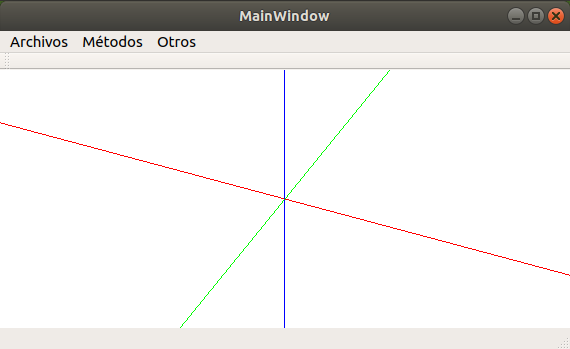
\includegraphics[width=0.7\linewidth]{UI}
			\caption{Aplicación desarrollada.}
		\end{figure} 
	\end{frame}

	\section{}
	\begin{frame}{Algunas referencias}
		\justifying
		\begin{thebibliography}{X}
			\bibitem{borwein} J.M. Borwein, A.S. Lewis, \textsl{Convex analysis and nonlinear optimization: theory and examples}, Second Edition, CMS Books in Mathematics/Ourrages Mathématiques de la SMC 3, Springer, New York, 2006.
			
			\bibitem{elliot1999mathematics} R.J. Elliot, R.E. Kopp, \textsl{Mathematics of financial markets}, Second Edition, Springer Finance, New York, 2005.
			
			\bibitem{giorgi2004mathematics} G. Giorgi, A. Guerraggio, J. Thierfelder, \textsl{Mathematics of optimization: smooth and nonsmooth case}, Elsevier Science B.V., Amsterdam, 2004.
			
			\bibitem{ICPBesl} Paul J.Besl y Neil D.McKay, \textsl{A method for registration of 3d-shapes}, IEEE Transactions on Pattern Analysis and Machine Inteligence, 1992.
			
			\bibitem{fischler1981random} Martin A Fischler y Robert C Bolles, \textsl{Random sample consensus: a paradigm for model fitting with applications to image analysis and automated cartography}, Communications of the ACM, 24(6):381–395, 1981.
			
			\bibitem{QuatYan} Yan-Bin Jia, \textsl{Quaternions and rotations}, Com S 477/577, 2013.
			Notes.
		
		\end{thebibliography}
	\end{frame}
	
\end{document}
